\chapter{Livello Data Link}
Per terminare la trattazione, vediamo il \emph{livello Data Link} e in particolare,
cerchiamo di capire quali sono i principi alla base dei servizi che offre
e come sono implementate alcune tra le più comuni tecnologie di \emph{livello
Data Link}.

\section{Introduzione}
Nella terminologia usata finora, \emph{\gls{glos:router}} e \emph{host} costituiscono
i nodi della rete e i canali di comunicazione tra due nodi sono detti \emph{link}
o \emph{collegamenti}. Abbiamo anche già detto che le \emph{\gls{glos:PDU}} di
\emph{livello Data Link} si chiamano \emph{frame} e incapsulano i \emph{pacchetti}
del \emph{livello Rete}. Diversamente da quanto visto finora, un \emph{frame},
oltre a \emph{header} e \emph{payload}, include anche un \emph{trailer} aggiunto
dopo il \emph{payload}. Mittente e destinatario sono identificati mediante
\emph{indirizzi \emph{\gls{glos:MAC}}}.

Lo scopo dei servizi di questo livello è trasportare i \emph{frame} da un nodo
a un altro fisicamente adiacente. Ovviamente, un percorso può attraversare più
\emph{collegamenti} che potrebbero anche utilizzare protocolli diversi.

\subsection{Servizi del livello Data Link}
Vediamo allora nel dettaglio quali sono i servizi offerti dal livello 2:
\begin{itemize}
    \item \emph{Consegna affidabile tra nodi adiacenti}: questo servizio è
    sempre implementabile, ma è poco usato su \emph{link} con bassi tassi di errore;
    \item \emph{Controllo di flusso}: la velocità di trasmissione viene adattata
    alle possibilità di mittente e destinatario;
    \item \emph{Rilevamento degli errori}: il ricevitore può identificare la presenza
    di errori ed agire di conseguenza;
    \item \emph{Correzione degli errori}: il ricevitore può identificare e
    correggere gli errori senza richiedere ritrasmissioni;
\end{itemize}
\noindent
Prima di procedere oltre, vediamo una caratterizzazione fondamentale dei
\emph{collegamenti}.
\begin{definition}[Collegamento half-duplex e full-duplex]
    Un collegamento nel quale i dati possono viaggiare in entrambe le direzioni
    contemporaneamente è detto essere full-duplex, altrimenti è half-duplex.
\end{definition}

\subsection{Implementazione dei servizi Data Link}
I servizi di livello 2 sono implementati su tutti gli \emph{host} e generalmente sono
gestiti dal firmware di un \quotes{adattatore di rete} o di un chip.
Questi componenti sono poi direttamente collegati al bus di sistema dell'\emph{host}.

\begin{note}
    L'implementazione del \emph{livello Data Link} richiede anche l'implementazione
    del \emph{livello Fisico}.
\end{note}\noindent
Il processo di trasmissione di un \emph{frame} è simile a quanto accade nei livelli
superiori: Il mittente incapsula i dati in un \emph{frame} e, se serve, aggiunge
ulteriori bit per il controllo degli errori e per il controllo di flusso; il
destinatario collabora al controllo di flusso\footnote{Vedremo più avanti come},
controlla la presenza di errori e quindi estrae i dati per passarli ai livelli
superiori.
\begin{figure}[h!]
    \centering
    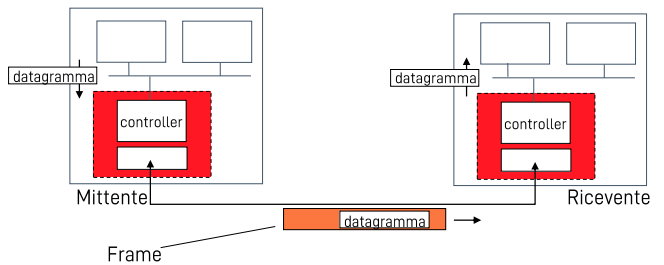
\includegraphics[width=0.7\textwidth]{trasmissione-data-link.png}
    \caption{Trasmissione di un \emph{frame} di livello 2}
\end{figure}

\section{Rilevamento e correzione di errori}
I meccanismi di rilevamento e correzione degli errori richiedono l'utilizzo di
bit ridondanti. Ad esempio, se EDC sono i bit ridondanti e D sono i dati da
proteggere, il processo di correzione e rilevamento di errori è a grandi linee
quello mostrato nella figura sottostante.

\begin{figure}[h!]
    \centering
    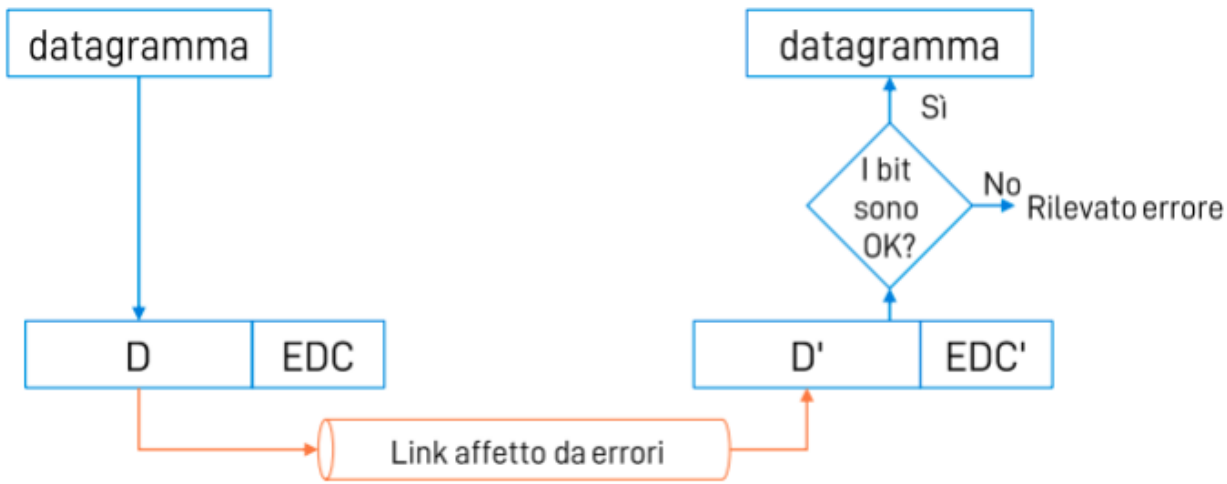
\includegraphics[width=0.7\textwidth]{rce.png}
    \caption{Meccanismo di rilevamento e controllo degli errori}
\end{figure}\noindent
Occorre però notare che il rilevamento degli errori non è mai affidabile al 100\%,
ma in generale, maggiore è la ridondanza, maggiore è la protezione.

\bigskip\noindent
Vediamo quindi alcuni algoritmi per il controllo e la correzione degli errori.

\subsection{Bit di parità}
Questa tecnica si può realizzare in una o due dimensioni. Nel primo caso viene
aggiunto un singolo bit che vale 1 se il numero di bit a 1 nella stringa
originale è dispari. La parità su due dimensioni prevede invece che a partire
dalla stringa di bit venga realizzata una matrice e che venga aggiunto un bit di
parità su ogni riga e ogni colonna.

Il controllo a una dimensione permette soltanto il rilevamento di errori, mentre il
controllo a due dimensioni permette anche la correzione.

\begin{figure}[h!]
    \centering
    \subfloat[Controllo a una dimensione]{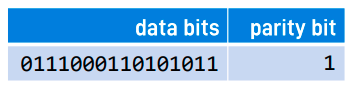
\includegraphics[width=0.3\textwidth]{partita1.png}}
    \subfloat[Controllo a due dimensioni]{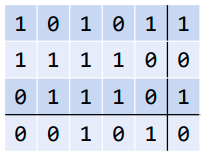
\includegraphics[width=0.3\textwidth]{partita2.png}}
    \subfloat[Controllo a due dimensioni con correzione]{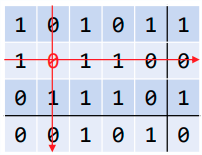
\includegraphics[width=0.3\textwidth]{partita3.png}}
    \caption{Controllo di parità}
\end{figure}\noindent
Il controllo di parità a due dimensioni permette di correggere gli errori solo se
in ogni riga e in ogni colonna si trova al più un bit errato. Comunque, in entrambe le
modalità, il rilevamento non funziona se il numero di bit sbagliati è pari.

\subsection{Ridondanza e interleaving}
Questa tecnica ridonda ogni bit della stringa e con un'operazione di interleaving
li riordina. Il risultato è una stringa di bit che resiste efficacemente a
raffiche di errori, ovvero a errori su bit in successione.

Quando il destinatario riceve i dati, ripristina l'ordine dei bit con un'operazione
di de-interleaving e ricostruisce il messaggio originale applicando una scelta a
maggioranza su gruppi di bit.

\begin{eg}[Esempio di applicazione]
    Si supponga di voler trasmettere la stringa \texttt{HELLO}. Ogni carattere viene
    ridondato ottenendo, ad esempio:
    \[\texttt{HHH EEE LLL LLL OOO}\]
    A questo punto con l'interleaving vengono riordinate le lettere:
    \[\texttt{HEL LOH ELL OHE LLO}\]
    Supponiamo quindi che una sequenza di 5 bit arrivi modificata al destinatario:
    \[\texttt{HEL LOH EXX XXX LLO}\]
    Dopo il riordino, il destinatario si ritrova la seguente stringa:
    \[\texttt{HHX EEX LXL LXL OXO}\]
    Scegliendo a maggioranza su ogni gruppo, si riesce comunque a ricostruire la stringa
    originale \texttt{HELLO}.
\end{eg}

\subsection{Cyclic Redundancy Check}
Il \emph{\gls{glos:CRC}} è attualmente l'algoritmo più efficiente per il controllo degli
errori. I dati vengono considerati come un numero binario $D$. L'algoritmo quindi, sceglie
una sequenza di $r+1$ bit detta \emph{\quotes{generatore}} e un altro numero $G$ noto sia
al mittente che al destinatario.

Quindi, il valore $R$ del \emph{CRC} viene composto scegliendo $r$ bit in modo tale che
$D\Mod{G}=R$ o, equivalentemente, che la concatenazione $\langle D,R\rangle\Mod{G}=0$. A
questo punto, se quando il destinatario calcola $\langle D,R\rangle\Mod{G}$ ottiene un
resto diverso da 0, c'è sicuramente un errore.

Questo sistema permette di rilevare anche errori a raffica, se questi hanno modificato meno
di $r$ bit in sequenza.

\begin{note}
    Per concatenare $D$ ed $R$ è sufficiente applicare la seguente funzione:
    \[\langle D,R\rangle=(D\cdot2^r)\texttt{ XOR }R\]
\end{note}

\paragraph{Calcolare il CRC}
Se $(D\cdot2^r)\texttt{ XOR }R$ deve essere un multiplo di $G$, deve valere
quanto segue:
\[(D\cdot2^r)\texttt{ XOR }R=n\cdot G\quad\text{con}\ n\in\mathbb{Z}\]
Applicando lo XOR a entrambi i membri, il termine a sinistra si semplifica:
\[D\cdot2^r=n\cdot G\texttt{ XOR }R\]
e segue che:
\[CRC=R=\texttt{resto}((D\cdot2^r)/G)=(D\cdot2^r)\Mod{G}\]

\begin{eg}[Esempio di calcolo del CRC]
    Supponiamo di aver ricevuto un messaggio $D=101110$ e di doverne verificare
    la correttezza. Siano $G=1001$ e $R=011$.

    \bigskip\noindent
    Iniziamo calcolando $D\cdot 2^r$. Poiché $R=011$ è una stringa di 3 bit,
    $r=3$ e quindi:
    \[D\cdot 2^r=101110000\footnotemark\]
    \footnotetext{Abbiamo semplicemente shiftato $D$ di 3 posizioni verso sinistra}
    Quindi, calcoliamo il CRC e vediamo se coincide col valore atteso.
    \begin{figure}[h!]
        \centering
        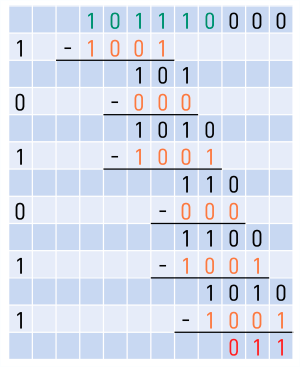
\includegraphics[width=0.28\textwidth]{calcolo-crc.png}
    \end{figure}

    \noindent
    Il resto è uguale ad $R$, quindi non ci sono stati errori e i dati sono
    corretti.
\end{eg}

\section{Gestione degli accessi multipli ai canali}
Distinguiamo due tipi di collegamenti:
\begin{itemize}
    \item \emph{Punto-punto}: sono collegamenti tra due soli \emph{host} e
    utilizzano protocolli per la comunicazione punto-punto (e.g. \emph{\gls{prot:PPP}});
    \item \emph{Broadcast}: sono collegamenti condivisi accessibili da più
    \emph{host};
\end{itemize}
I \emph{collegamenti broadcast} comportano una serie di problemi legati alla
necessità di regolare le trasmissioni ed evitare le interferenze. Infatti, se
due o più \emph{host} trasmettessero nello stesso momento, i segnali delle
rispettive trasmissioni si mescolerebbero tra loro. Se invece un \emph{host}
ricevesse due o più trasmissioni nello stesso momento, si verificherebbe una
\emph{collisione}.

Per evitare ciò, vengono usati protocolli di accesso multiplo, ovvero algoritmi
distribuiti che determinano il modo e il momento in cui ogni \emph{host} può
trasmettere su un canale. Le informazioni necessarie per il funzionamento dei
protocolli possono viaggiare sullo stesso canale dei dati o su un canale dedicato
e in quel caso si parla di \emph{\quotes{out-of-band} channel}.

Idealmente, vorremmo che in un \emph{collegamento} a $R\frac{bit}{s}$, il
protocollo \emph{\gls{prot:MACp}} utilizzato permetta ad un \emph{host} di usare
l'intera \emph{banda}, quando è l'unico a trasmettere, o che questa venga divisa
equamente tra tutti gli \emph{host} che vogliono trasmettere. Inoltre, il
protocollo dovrebbe essere semplice e funzionare in modo decentralizzato.

A questo punto possiamo suddividere i protocolli \emph{MAC} in tre categorie:
\begin{enumerate}
    \item \emph{Protocolli a ripartizione delle risorse}: le risorse di un
    canale vengono suddivise equamente tra tutti gli \emph{host} ad esso connesse;
    \item \emph{Protocolli ad accesso casuale}: il canale non viene suddiviso, ma
    si cerca di limitare il numero di \emph{collisioni};
    \item \emph{Protocolli a turni intelligenti}: gli \emph{host} accedono al
    canale a turno e la durata dei turni varia in base alla quantità di dati da
    trasmettere;
\end{enumerate}

\subsection{Protocolli a ripartizione di risorse}
All'interno di questa classe consideriamo tre protocolli: \emph{\gls{prot:TDMA}},
\emph{\gls{prot:FDMA}} e \emph{\gls{prot:CDMA}}.
All'inizio della trattazione abbiamo già descritto i principi di \emph{TDMA} e
\emph{FDMA}. Nel primo vengono definiti degli slot temporali di dimensione fissa
che vengono assegnati agli \emph{host}. Gli \emph{host} trasmettono con un
sistema a turni e utilizzano tutta la banda disponibile. Nel caso dell'\emph{FDMA}
invece, lo spettro del canale viene suddiviso in sotto-bande che vengono assegnate
ai trasmettitori. Ogni \emph{host} può quindi trasmettere in qualsiasi momento e
senza limiti di tempo. In entrambi i casi però, quando un \emph{host} non ha
bisogno di trasmettere, le risorse ad esso assegnate rimangono inutilizzate.

Diverso è invece il funzionamento del \emph{CDMA}, nel quale, ogni \emph{host}
può usare tutta la banda e tutto il tempo e la ripartizione delle risorse
avviene assegnando un \quotes{codice} diverso ad ogni \emph{host}. Con codice
si intende una sequenza di bit detti \quotes{chip} che commuta più rapidamente
di quanto commutino i bit di dati. Quando un \emph{host} trasmette, trasmette lo
\texttt{XOR} tra la sequenza dei dati e il codice. Il ricevente ricalcolando lo
\texttt{XOR} con lo stesso codice, riesce a recuperare i dati originali. Se
invece la stringa ricevuta venisse \quotes{xorata} con un codice diverso, il
risultato non avrebbe alcun significato.

\begin{figure}[ht]
    \centering
    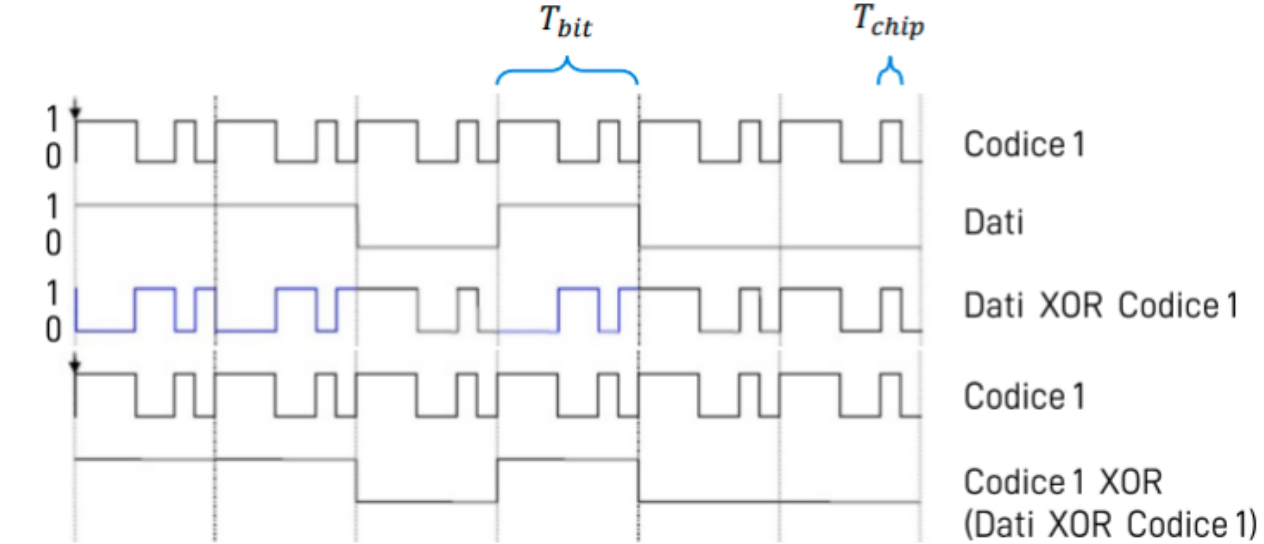
\includegraphics[width=0.85\textwidth]{cdma1.png}
    \caption{Funzionamento del \emph{CDMA}}
\end{figure}

Il problema di questa tecnica è che poiché il codice deve commutare più
velocemente dei dati, ovvero $T_\emph{chip}>T_\emph{bit}$, è necessario
diminuire la velocità di trasmissione dei dati, di fatto, rallentando la
comunicazione.

\begin{figure}[ht!]
    \centering
    \subfloat[\emph{TDMA}]{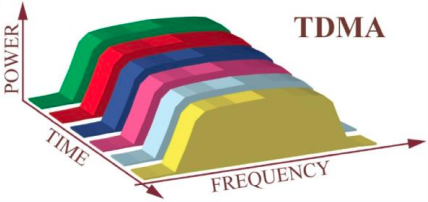
\includegraphics[width=0.32\textwidth]{tdma1.png}}
    \hspace{1mm}
    \subfloat[\emph{FDMA}]{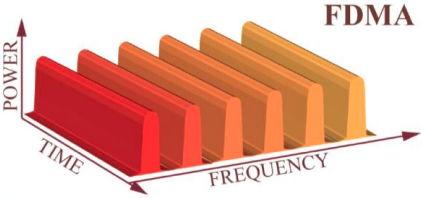
\includegraphics[width=0.32\textwidth]{fdma1.png}}
    \hspace{1.5mm}
    \subfloat[\emph{CDMA}]{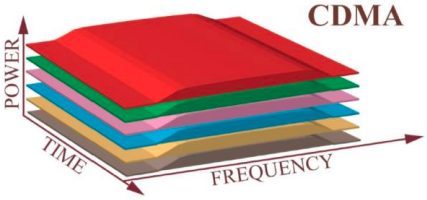
\includegraphics[width=0.32\textwidth]{cdma2.png}}
    \caption{Confronto tra protocolli a ripartizione di risorse}
\end{figure}

\subsection{Protocolli ad accesso casuale}
I protocolli ad accesso casuale prevedono che quando un \emph{host} trasmette,
lo faccia con la banda massima possibile. Non prevedono alcun coordinamento tra
gli \emph{host} prima della trasmissione e, di conseguenza, si possono verificare
delle \emph{collisioni}. Sono poi i protocolli stessi a stabilire come e se
rilevare e recuperare le \emph{collisioni}.

\paragraph{Slotted ALOHA}
Nello \emph{Slotted ALOHA} tutti i \emph{frame} sono della stessa lunghezza e il
tempo viene suddiviso in slot di durata pari alla dimensione dei \emph{frame}.
Tutti gli \emph{host} sono sincronizzati e possono trasmettere solo all'inizio
di uno slot. Nel caso di \emph{collisioni}, queste vengono rilevate da tutti
gli \emph{host} che stanno trasmettendo.

A questo punto il funzionamento è molto semplice: quando un \emph{host} deve
trasmettere, aspetta l'inizio dello slot successivo. Se non ci sono
\emph{collisioni}, continua a trasmettere anche nello slot seguente altrimenti,
con probabilità $p$, ritrasmette nello slot successivo finché non ha successo.

\begin{figure}[h!]
    \centering
    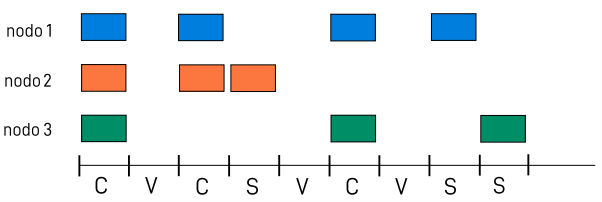
\includegraphics[width=0.65\textwidth]{slotted-aloha-1.png}
    \caption{Funzionamento dello \emph{Slotted ALOHA}}
\end{figure}

\noindent
I vantaggi di questo protocollo sono la semplicità di implementazione, la
decentralizzazione e la possibilità per un \emph{host} di trasmettere in
continuazione nel caso sia l'unico a doverlo fare. Tuttavia, la sincronizzazione
richiede un coordinamento, alcuni slot potrebbero rimanere inutilizzati e le
\emph{collisioni} sono probabili e frequenti. Inoltre, questa modalità di
rilevamento delle \emph{collisioni} costringe ad aspettare la fine della
trasmissione introducendo un'inefficienza di fondo.

\bigskip\noindent
Proviamo allora a calcolare l'efficienza di questo protocollo.

Tutti i \emph{frame} hanno la stessa dimensione. Chiamiamo $G$ il traffico
offerto, cioè il numero medio di \emph{frame} inviati sul canale da tutti gli
\emph{host}, includendo sia trasmissioni che ritrasmissioni. Ovviamente $G\geq0$.
La probabilità che in uno slot ci siano $k$ \emph{frame} da trasmettere è
descritta dalla seguente variabile aleatoria di Poisson:
\[P[k]=\frac{G^k\cdot e^{-G}}{k!}\]
Il \emph{throughput} ideale è 1 poiché nella situazione migliore in ogni slot
c'è soltanto un \emph{frame} da inviare rendendo impossibile il verificarsi di
\emph{collisioni}. Il \emph{throughput} effettivo corrisponde invece al valore
di $P[k=1]$:
\[P[k=1]=G\cdot e^{-G}\]
Il valore massimo di questa funzione si ottiene quando $G^*=1$. Sostituendo quel
valore nella funzione di probabilità si ottiene un \emph{throughput} massimo
pari a $\frac{1}{e}\approx0.368$.

\paragraph{ALOHA}
L'\emph{ALOHA}, o \emph{ALOHA puro}, funziona come lo \emph{Slotted ALOHA}, ma
gli \emph{host} non sono sincronizzati e quindi i \emph{frame} vengono trasmessi
immediatamente e non all'inizio di uno slot.

Il prezzo di questa maggiore semplicità lo si paga in efficienza in quanto la
probabilità di \emph{collisione} aumenta: un \emph{frame} inviato al tempo $t_0$
collide con i \emph{frame} inviati nell'intervallo $[t_0-1,\,t_0+1]$.

\begin{figure}[h!]
    \centering
    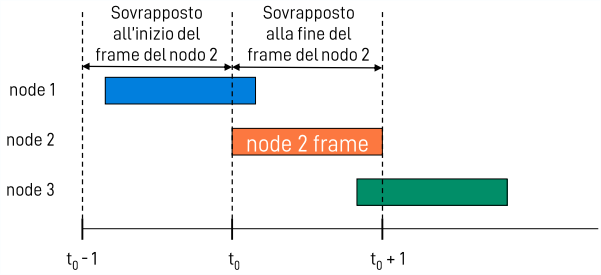
\includegraphics[width=0.65\textwidth]{aloha-1.png}
    \caption{Funzionamento dell'\emph{ALOHA}}
\end{figure}

\bigskip\noindent
Proviamo a calcolare l'efficienza di questa versione. Le supposizioni solo le
stessa fatte in precedenza, tranne per il \emph{throughput} che stavolta corrisponde
alla probabilità che un \emph{frame} venga trasmesso all'interno dell'intervallo
di vulnerabilità $[t_0-1,\,t_0+1]$.

Quindi, la probabilità che al tempo $t$ venga trasmesso un solo \emph{frame} è:
\[P[k=1]=G\cdot e^{-G}\]
La probabilità che non ci siano \emph{frame} la cui trasmissione è iniziata
nell'intervallo $[t_0,\,t]$ vale invece:
\[P[k=0]=e^{-G}\]
La probabilità che una trasmissione abbia successo vale quindi:
\[P[k=1]\cdot P[k=0]=(G\cdot e^{-G})\cdot e^{-G}=G\cdot e^{-2G}\]
Questa funzione ha valore massimo quando $G=\frac{1}{2}$ e quindi il
\emph{throughput} massimo è pari a $\frac{1}{2e}\approx0.184$ che è la metà
del \emph{throughput} massimo dello \emph{Slotted ALOHA}.

\begin{figure}[h!]
    \centering
    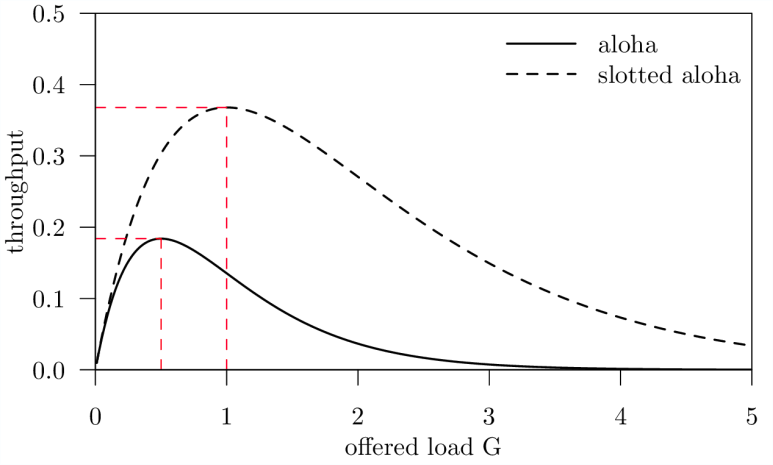
\includegraphics[width=0.8\textwidth]{aloha-vs-slotted.png}
    \caption{Confronto tra \emph{Slotted ALOHA} e \emph{ALOHA}}
\end{figure}

\paragraph{CSMA}
Il \emph{\gls{prot:CSMA}} è un protocollo basato sull'ascolto. In particolare,
viene \quotes{ascoltato} il canale e, se è libero, viene trasmesso un
\emph{frame}, altrimenti viene ritardata la trasmissione. Esistono diverse
versioni del protocollo che si distinguono in base al comportamento in caso di
canale occupato.
\begin{itemize}
    \item \emph{CSMA 0-persistente}: se il canale è occupato l'\emph{host}
    attende un tempo casuale maggiore del tempo di trasmissione e poi ritenta;
    \item \emph{CSMA 1-persistente}: se il canale è occupato l'\emph{host}
    attende fino a quando non si libera e poi trasmette;
    \item \emph{CSMA p-persistente}: se il canale è occupato l'\emph{host}
    attende fino a quando non si libera e poi con probabilità $p$ trasmette il
    \emph{frame} e con probabilità $1-p$ attende un tempo casuale maggiore del
    tempo di trasmissione prima di ritentare;
\end{itemize}
In tutti e tre i casi, se si verifica una \emph{collisione}, l'\emph{host}
rimane in attesa per un tempo casuale e poi ritenta secondo quelle che sono le
procedure utilizzate.

\begin{figure}[ht!]
    \centering
    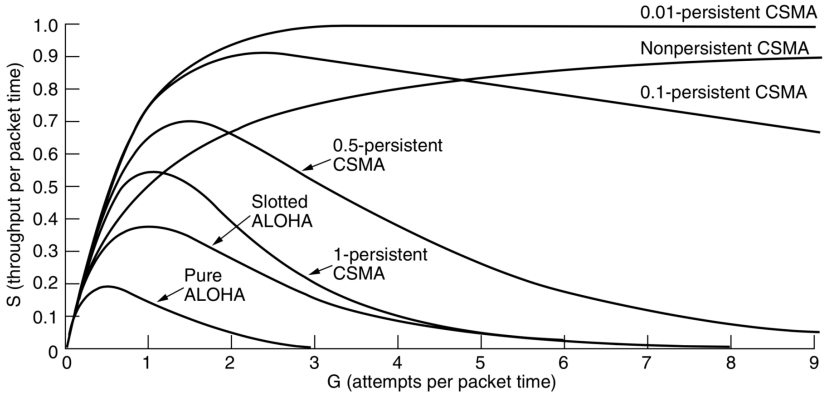
\includegraphics[width=0.8\textwidth]{confronto-csma.png}
    \caption{Confronto tra le versioni del \emph{CSMA}}
\end{figure}

\newpage\noindent
Come fa il \emph{CSMA} a gestire le collisioni?

Consideriamo il periodo di vulnerabilità. Esso dipende dal \emph{tempo di
propagazione} $\tau$ e dal tempo richiesto $T_a$ per rilevare se il canale è
libero o meno. Se un \emph{host} trasmette, ma il segnale non ha raggiunto tutti
gli altri \emph{host}, qualcun altro potrebbe iniziare a trasmettere. La finestra
temporale all'interno della quale ciò potrebbe accadere corrisponde al periodo
di vulnerabilità $T_v=\tau+T_a$. Per questo motivo, il \emph{CSMA} solitamente
si usa quando il \emph{tempo di propagazione} è molto minore del \emph{tempo di
trasmissione}.

\begin{figure}[h!]
    \centering
    \subfloat{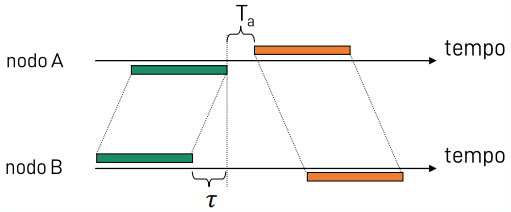
\includegraphics[width=0.51\textwidth, valign=c]{vulnerabilita-csma.png}}
    \hfill
    \subfloat{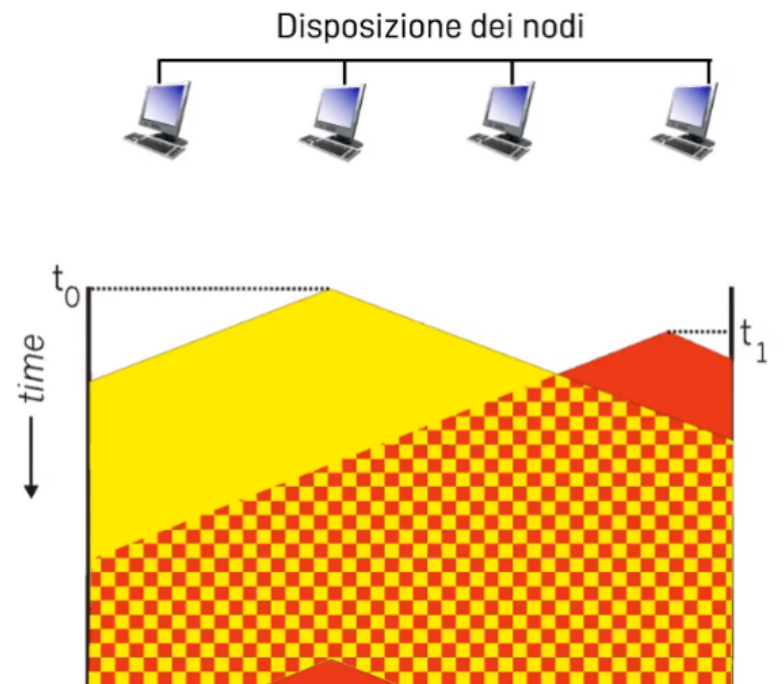
\includegraphics[width=0.43\textwidth, valign=c]{collisione-csma-2.png}}
    \caption{\emph{Periodo di vulnerabilità} e \emph{collisioni} nel \emph{CSMA}}
\end{figure}\noindent
Quindi, nel \emph{CSMA} il \emph{ritardo di propagazione} porta al verificarsi
di \emph{collisioni}. Quando ciò accade, l'intero \emph{tempo di trasmissione}
viene sprecato.

Per questo motivo esistono due ulteriori versioni del \emph{CSMA}: \emph{
\gls{prot:CSMACD}} e \emph{\gls{prot:CSMACA}} che permettono rispettivamente di
rilevare ed evitare le \emph{collisioni}. Il primo è in grado di rilevare le
\emph{collisioni} e quindi di interrompere la trasmissione riducendo lo spreco
di risorse. Nel secondo invece, il funzionamento è uguale a quello che si ha
nel \emph{CSMA p-persistente}, ma il parametro $p$ viene fatto variare in base
alle condizioni della rete.

Il motivo per il quale esistono sia il \emph{CSMA/CD} che il \emph{CSMA/CA} è
che il rilevamento delle \emph{collisioni} viene fatto confrontando la potenza
del segnale trasmesso con quella del segnale ricevuto. Questo confronto è molto
difficile nel caso delle reti wireless in quanto la potenza del segnale trasmesso
è molto maggiore della potenza del segnale ricevuto. Quindi, il \emph{CSMA/CD}
è usato nelle reti cablate, mentre il \emph{CSMA/CA} nelle reti wireless nelle
quali, inoltre, il \emph{tempo di trasmissione} è molto minore del \emph{tempo
di propagazione} $\tau$ e del tempo $T_a$ necessario per sondare il canale,
ovvero: $T<<\tau+T_a$

\begin{figure}[h!]
    \centering
    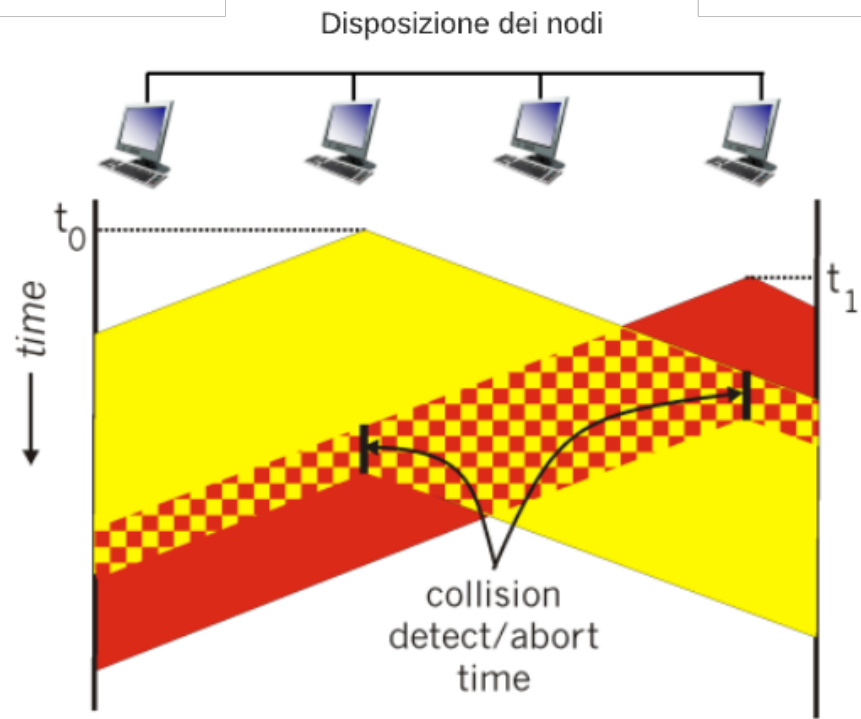
\includegraphics[width=0.5\textwidth]{csma-cd.png}
    \caption{Comportamento del \emph{CSMA/CD}}
\end{figure}

\subsection{Protocolli a turni intelligenti}
\paragraph{Polling}
È un protocollo basato sul paradigma \emph{master-slave} nel quale un \emph{host},
il \emph{master}, invita gli altri \emph{host}, gli \emph{slave}, a trasmettere
a turno. Di solito è usato in reti nella quali gli \emph{slave} hanno una
bassa potenza di calcolo. Nonostante l'evidente semplicità, si hanno problemi
legati all'alta latenza, all'overhead provocato dai messaggi di polling e alla
presenza di un \emph{\gls{glos:SPOF}}.

\paragraph{Token passing}
Esiste un \emph{token}, un particolare \emph{frame}, che conferisce
all'\emph{host} che ne è in possesso il diritto a trasmettere. Il \emph{token}
viene quindi fatto girare tra tutti gli \emph{host} permettendo a tutti, prima
o poi, di trasmettere. I problemi di questo protocollo sono gli stessi del
precedente e in particolare, il \emph{SPOF} è costituito dal \emph{token}.

\begin{figure}[h!]
    \centering
    \hspace{-0.5cm}
    \subfloat[\emph{Polling}]{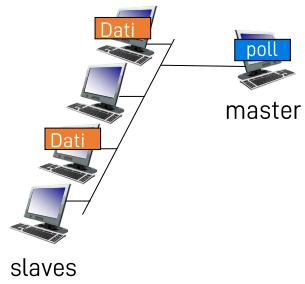
\includegraphics[width=0.3\textwidth]{polling.png}}
    \hspace{3cm}
    \subfloat[\emph{Token passing}]{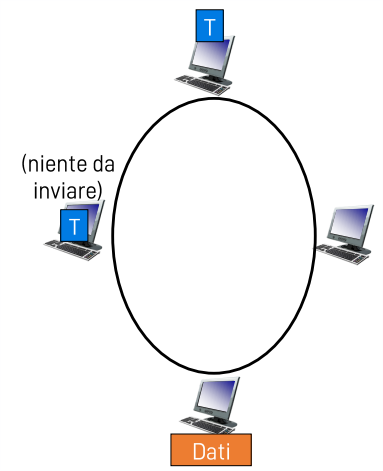
\includegraphics[width=0.28\textwidth]{token.png}}
    \caption{\emph{Polling} e \emph{Token passing}}
\end{figure}

\section{Protocollo Ethernet}
I protocolli del \emph{livello Data Link} e del \emph{livello Fisico} sono
standardizzati e appartengono al gruppo \emph{IEEE 802}.
\begin{figure}[h!]
    \centering
    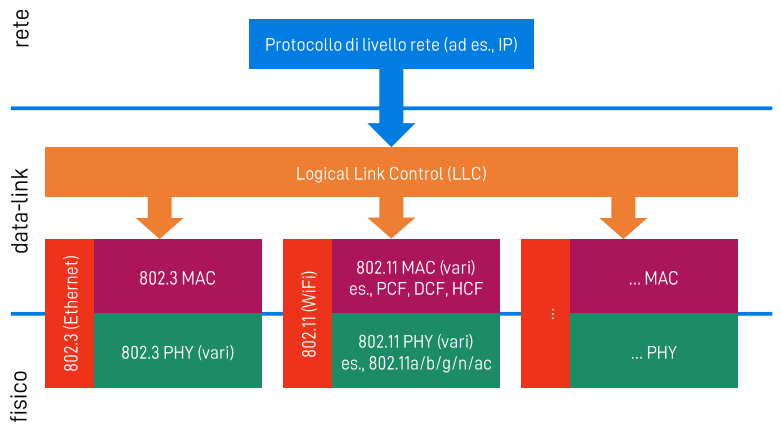
\includegraphics[width=0.8\textwidth]{ieee802.png}
    \caption{Protocolli del gruppo \emph{IEEE 802}}
\end{figure}

\begin{note}
    Ogni protocollo del \emph{livello Data Link} è associato ai rispettivi
    protocolli di \emph{livello Fisico}.
\end{note}\noindent
Nelle reti cablate il protocollo che di fatto è lo standard universale è il
protocollo \emph{Ethernet}. \emph{Ethernet} nasce come protocollo proprietario
col nome \emph{DIX Ethernet} (Digital-Intel-Xenox) per poi essere standardizzato
e liberalizzato.

\subsection{Organizzazione delle reti Ethernet}
Inizialmente le reti \emph{Ethernet} erano organizzate secondo la topologia a
bus e quindi vi era un unico mezzo di trasmissione condiviso al quale,
mediante un \emph{transceiver}, si collegavano tutti gli \emph{host} di quella
rete. I dati trasmessi da un \emph{host} venivano ricevuti da tutti.

\begin{figure}[h!]
    \centering
    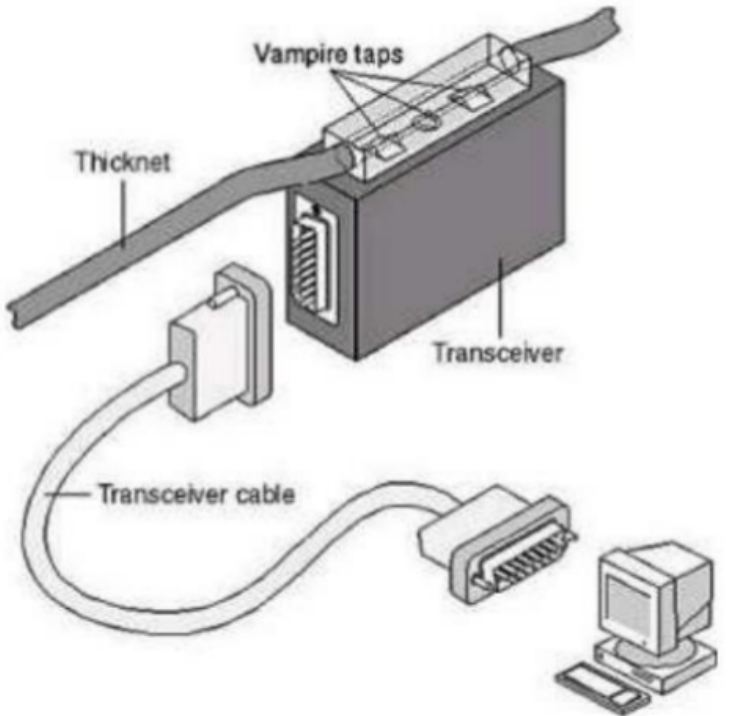
\includegraphics[width=0.425\textwidth]{transceiver.png}
    \caption{\emph{Transceiver Ethernet}}
\end{figure}

\begin{figure}[ht!]
    \centering
    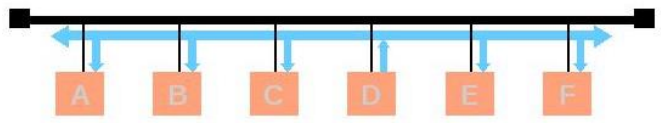
\includegraphics[width=0.8\textwidth]{ethernet-bus.png}
    \caption{Rete \emph{Ethernet} con topologia a bus}
\end{figure}

\begin{figure}[ht!]
    \centering
    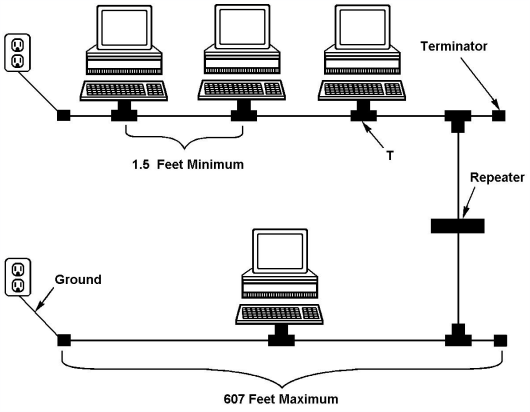
\includegraphics[width=0.8\textwidth]{organizzazione-bus.png}
    \caption{Organizzazione di una rete \emph{Ethernet} a bus}
\end{figure}

\noindent
Il terminatore (Terminator nella figura sopra) è necessario per evitare che il
segnale, raggiunta la fine del cavo, ritorni indietro.

Con la nascita degli hub prima e degli \emph{\gls{glos:switch}} dopo la
topologia a bus è stata sostituita da quella a stella. In questa topologia,
tutti gli \emph{host} sono collegati ad un dispositivo centrale che riceve
tutti i \emph{frame} e li inoltra ad uno o più degli altri \emph{host}.

\subsection{Struttura dei frame Ethernet}
Le schede di rete, nel momento dell'invio, incapsulano i \emph{pacchetti} di
livello 3 all'interno di \emph{frame} di livello 2. Nel caso del protocollo
\emph{Ethernet} la struttura dei \emph{frame} è quella descritta nella figura
sottostante.
\begin{figure}[h!]
    \centering
    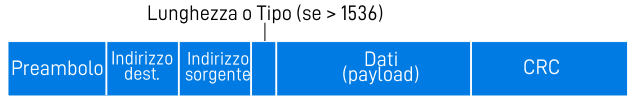
\includegraphics[width=0.8\textwidth]{frame-ethernet.png}
    \caption{Campi di un \emph{frame Ethernet}}
\end{figure}

\bigskip\noindent
Esaminiamo i singoli campi:
\begin{itemize}
    \item \texttt{Preambolo}: è composto da 7 byte \texttt{10101010} e un byte
    \texttt{10101011} ed è utilizzato per sincronizzare il clock del ricevitore
    e del trasmettitore;
    \item \texttt{Indirizzo destinazione}: un gruppo di 6 byte con i quali è
    rappresentato l'\emph{indirizzo MAC} di destinazione;
    \item \texttt{Indirizzo sorgente}: un gruppo di 6 byte con i quali è
    rappresentato l'\emph{indirizzo MAC} sorgente;
    \item \texttt{Lunghezza}: è un valore a 16 bit che indica la dimensione
    in byte dell'intero \emph{frame};
    \item \texttt{Tipo}: identifica il protocollo di livello 3 trasportato;
    \item \texttt{Dati}: è il \emph{payload} del \emph{frame};
    \item \texttt{CRC}: codice per effettuare il controllo degli errori con
    l'algoritmo \emph{\gls{glos:CRC}};
\end{itemize}
\begin{note}
    L'indirizzo di destinazione è il secondo campo del \emph{frame} in modo
    che sia possibile prendere decisioni di inotro concorrenzialmente alla
    ricezione dei restanti byte. Il codice \emph{CRC} invece,
    è in fondo al \emph{frame} perché per eseguire i controlli d'errore è
    necessario averlo prima ricevuto per intero.
\end{note}
\noindent
Quando una scheda di rete riceve un \emph{frame} diretto a sé oppure un
\emph{frame} con un indirizzo di \emph{broadcast}, passa il \emph{payload} del
\emph{frame} al livello superiore, altrimenti scarta tutto il \emph{frame}.

\subsection{Caratteristiche del protocollo Ethernet}
Il protocollo \emph{Ethernet} non è né un protocollo connesso, per cui non avviene
alcuno scambio di messaggi di controllo tra mittente e destinatario, e né un
protocollo affidabile. Non vengono infatti usati messaggi \emph{ACK}
o simili per gestire le ritrasmissioni e l'unico controllo che viene fatto è
mediante il \emph{CRC}. Di conseguenza, eventuali ritrasmissioni vengono gestite
dai protocolli di livello superiore.

\emph{Ethernet} implementa un protocollo \emph{\gls{prot:MACp}} di tipo
\emph{CSMA/CD \quotes{unslotted}}. Ciò significa che quando la scheda di rete
ha un \emph{frame} da trasmettere, verifica lo stato del canale: se è libero
trasmette, altrimenti trasmette appena possibile. Se la trasmissione termina
senza rilevare altre trasmissioni, il \emph{frame} viene considerato consegnato.
In caso contrario, la scheda trasmette un segnale di \quotes{abort}.
Ogni volta che si verifica una \emph{collisione}, la scheda sceglie a caso un
valore di backoff, cioè il tempo che deve attendere prima di riprovare a trasmettere,
tra i valori 0 e $(2^k-1)T$ dove $k\leq7$ e $T$ è un valore noto (e.g. $50\mu s$)
che rappresenta il tempo necessario a trasmettere 512 bit.

\begin{note}
    Il valore di backoff può essere soltanto 0 o $(2^k-1)T$ e non un
    valore intermedio.
\end{note}
\begin{note}
    Sebbene esistano molti standard \emph{Ethernet} differenti, la struttura dei
    \emph{frame} e i protocolli \emph{MAC} sono comuni.
\end{note}

\section{Ethernet switching}
In precedenza abbiamo parlato di dispositivi quali hub e \emph{switch}. Un hub
non è altro che un ripetitore: ogni volta che riceve un \emph{frame} lo inoltra,
senza fare altro, su tutte le porte ad eccezione di quella di arrivo. Uno
\emph{switch} d'altra parte, è un dispositivo più attivo: quando riceve un
\emph{frame}, esamina l'\emph{indirizzo MAC} di destinazione e seleziona di
conseguenza le porte verso le quali inoltrarlo. Inoltre, gli \emph{switch}
sono trasparenti agli altri \emph{host} e sono in grado di configurarsi
automaticamente, cioè possono associare ad ogni porta gli \emph{indirizzi MAC}
dei dispositivi da essa raggiungibili.

\subsection{Domini di collisione}
\begin{definition}[Dominio di collisione]
    Un dominio di collisione rappresenta la porzione di rete all'interno della
    quale possono verificarsi delle collisioni.
\end{definition}\noindent
La scelta della topologia e la scelta dei dispositivi di rete influenzano il
numero dei \emph{domini di collisione}. Utilizzando una topologia a bus, tutti
gli \emph{host} connessi al canale appartengono allo stesso \emph{dominio} e quindi
ogni \emph{host} può collidere con qualunque altro. Nella topologia a stella
invece, va considerato il dispositivo che funge da centro: se si tratta di un
hub, esiste un unico \emph{dominio}, mentre con uno \emph{switch} si ottengono
tanti \emph{domini} quante sono le porte dello \emph{switch} utilizzate.
Ciò significa che ogni \emph{host} comunica con lo \emph{switch} su un canale
dedicato e quindi, se il \emph{collegamento} è di tipo \emph{full duplex}, non
si possono verificare \emph{collisioni}. Inoltre, questo permette anche
a coppie di \emph{host} di comunicare simultaneamente.

\begin{figure}[h!]
    \centering
    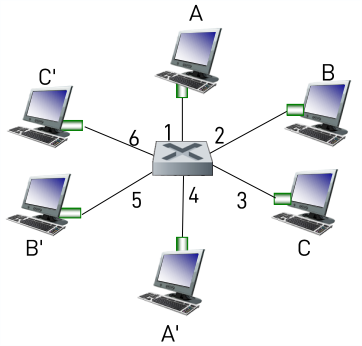
\includegraphics[width=0.5\textwidth]{switch-1.png}
    \caption{Rete \quotes{switched}}
\end{figure}\noindent
Ad esempio, nella figura di cui sopra, le comunicazioni tra $A$ e $A'$ e tra
$B$ e $B'$ possono avvenire in contemporanea senza che si verifichino
\emph{collisioni}.

\subsection{Domini di broadcast}
\begin{definition}[Dominio di broadcast]
    Un dominio di broadcast rappresenta la porzione di rete all'interno della
    quale può viaggiare un messaggio broadcast di livello 2.
\end{definition}\noindent
È importante ricordare che ad ogni \emph{dominio di collisione} può corrispondere
un solo \emph{dominio di broadcast}. Il motivo è che se un \emph{dominio di
collisione} si estendesse su due \emph{domini di broadcast}, i messaggi
trasmessi in broadcast dall'\emph{ARP} non potrebbero raggiungere tutti gli
\emph{host} necessari e quindi si creerebbero due gruppi di \emph{host}
irraggiungibili.

\begin{note}
    Ogni interfaccia di un \emph{router} definisce un \emph{dominio di
    broadcast}.
\end{note}

\begin{figure}[ht!]
    \centering
    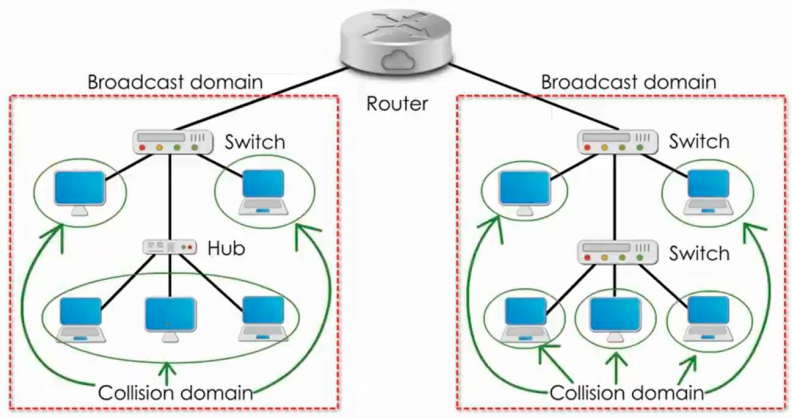
\includegraphics[width=0.8\textwidth]{collisione-vs-broadcast.png}
    \caption{\emph{Domini di collisione} e \emph{di broadcast} in una rete}
\end{figure}

\subsection{Funzionamento degli switch}
A questo punto ci chiediamo come facciano gli \emph{switch} ad autoconfigurarsi
e prendere le decisioni di inoltro. Come sarà facile immaginare, gli \emph{switch}
mantengono una tabella di questo tipo:

\begin{figure}[h!]
    \centering
    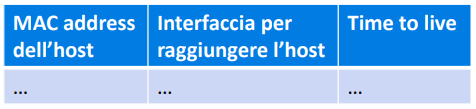
\includegraphics[width=0.5\textwidth]{switch-tabella-1.png}
    \caption{Tabella di inoltro di uno \emph{switch}}
\end{figure}\noindent
Il \texttt{Time to live} serve per mantenere aggiornate le entry scartando
quelle troppo vecchie.

Configurare uno \emph{switch} significa popolare la suddetta tabella e il
processo che consente ai dispositivi di autoconfigurarsi è chiamato
\emph{backward learning}. In pratica, quando uno \emph{switch} riceve un
\emph{frame}, aggiorna la tabella di inoltro, inserendo o aggiornando l'entry
associata all'\emph{indirizzo MAC} sorgente quindi, ricerca nella tabella
l'\emph{indirizzo MAC} di destinazione del \emph{frame}: se
l'entry esiste e l'interfaccia di uscita è diversa da quella di arrivo, inoltra
il \emph{frame}, altrimenti lo scarta. Se invece non viene trovata alcuna
corrispondenza, il \emph{frame} viene trasmesso in \emph{flooding} su tutte
le interfacce.

\begin{note}
    Il motivo per il quale gli \emph{switch} scartano i \emph{frame} che
    dovrebbero essere inoltrati verso le stessa interfaccia di quella di arrivo
    è che, se è ciò accade, significa che a quella interfaccia è collegato un
    hub al quale sono collegati sia l'\emph{host} sorgente che il destinatario.
    Di conseguenza, il \emph{frame} ricevuto è già stato inviato dall'hub
    verso il legittimo destinatario e quindi se lo \emph{switch} inoltrasse il
    \emph{frame}, l'hub non farebbe altro che ritrasmetterlo di nuovo in
    \emph{flooding} con la conseguenza che il destinatario riceverebbe due volte
    lo stesso \emph{frame}.
\end{note}

\subsection{Protocollo STP}
Il processo di \emph{backward learning} funziona anche con configurazioni più
complesse degli apparati di rete. L'unica situazione nella quale si
riscontrerebbero problemi è quella in cui esistono dei cicli tra gli \emph{switch}.

\begin{eg}[Esempio di creazione di un ciclo]
    Consideriamo per esempio la seguente configurazione:

    \begin{figure}[h!]
        \centering
        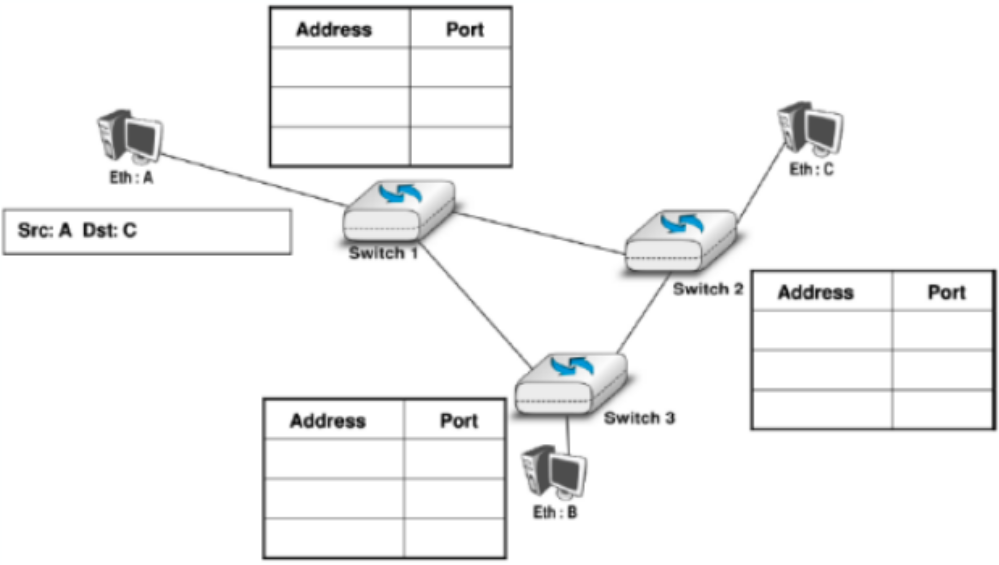
\includegraphics[width=0.57\textwidth]{switch-ciclo.png}
    \end{figure}\noindent
    Supponiamo che $A$ debba inviare un frame a $C$. $Switch 1$ riceve il frame
    e non sapendo a chi inoltrarlo, lo trasmette in flooding. A questo punto,
    sia $Switch 2$ che $Switch 3$ ricevono il frame e di nuovo provano ad
    inviarlo in flooding. Sebbene con questo secondo passaggio il frame riesca
    ad arrivare alla sua destinazione, copie di esso continueranno a circolare
    potenzialmente all'infinito.
\end{eg}\noindent
È evidente che questo problema può portare velocemente a saturare la capacità
dei \emph{collegamenti}. La soluzione a ciò è l'\emph{\gls{prot:STP}}. L'\emph{STP}
prevede che tutti gli \emph{switch} siano identificati per mezzo di un valore a
64 bit formato in modo tale che i primi 16 bit sono configurati
dall'amministratore di reti, mentre i restanti 48 bit sono l'\emph{indirizzo MAC}
dello \emph{switch}. Il protocollo a quel punto costruisce un albero con radice
nello \emph{switch} con ID minore. Questa modalità di scelta della radice
permette all'amministratore di sceglierla nel modo più consono all'organizzazione
della proprio rete.

\paragraph{Processo di costruzione dell'albero di copertura}
Per creare l'albero di copertura gli \emph{switch} si scambiano messaggi di
controllo chiamati \emph{\gls{glos:BPDU}} che contengono l'ID del mittente e il
costo del \emph{collegamento}. Quando uno \emph{switch} $A$ riceve una \emph{BPDU}
da un altro \emph{switch} $B$, se l'ID di $A$ è minore dell'ID di $B$, la porta
di $B$ verso $A$ diventa la radice dell'albero per $B$, ovvero $A$ diventa il
padre di $B$ nell'albero. Se invece l'ID di $A$ è maggiore, la porta sulla quale
$A$ ha ricevuto il messaggio diventa la radice dell'albero per $A$ e quindi $B$
diventa padre di $A$ nell'albero.

Se $A$ diventa radice di $B$, $A$ aggiorna il proprio costo a $c=cost_A+cost_B$
e tutte le porte dalle quali $A$ riceve \emph{BPDU} con costo maggiore di $c$
vengono identificate come \emph{\quotes{designated ports}}, cioè figli di $A$
nell'albero. I messaggi provenienti invece da porte il cui costo è uguale a $c$
diventano \emph{\quotes{blocked ports}} perché quelle porte sono potenziali
padri di $B$ e creerebbero cicli ai livelli più alti dell'albero se venissero
usate.

\bigskip\noindent
Al termine del processo, ogni porta di collegamento tra \emph{switch} sarà
stata associata ad uno dei tre possibili tipi:
\begin{table}[ht!]
    \centering
    \renewcommand{\arraystretch}{1.2}
    \begin{tabular}{|c|c|c|c|}
        \hline
        \textbf{Tipo} & \textbf{Può ricevere BPDU} & \textbf{Può inviare BPDU}
        & \textbf{Può gestire i frame}\\
        \hline
        Blocked & Sì & No & No\\
        \hline
        Radice & Sì & No & Sì\\
        \hline
        Designated & Sì & Sì & Sì\\
        \hline
    \end{tabular}
\end{table}

\paragraph{Variazioni dell'albero di copertura}
Le \emph{BDPU} vengono inviate periodicamente per rilevare cambiamenti, ma ogni
\emph{switch} le trasmette soltanto verso le \emph{\quotes{designated ports}}.
In particolare, lo \emph{switch} radice trasmette una \emph{BPDU} verso tutte
le proprie \emph{\quotes{designated ports}} e gli altri \emph{switch} a loro
volta fanno lo stesso. Ogni \emph{switch} poi, tiene traccia del momento in
cui ha ricevuto l'ultima \emph{BPDU}. Passato un certo periodo il processo di
formazione dell'albero di copertura riparte da zero e fino a quando non si
conclude gli \emph{switch} non inoltrano il normale traffico dati.

\subsection{Organizzazione logica delle LAN}
Suddividere gli \emph{host} di una \emph{\gls{glos:LAN}} in gruppi è spesso una
buona idea. Sia per ridurre le dimensioni dei \emph{domini di broadcast} e
aumentare così l'efficienza della rete, che per ridurre il carico di alcune
porzioni di rete più sensibili. Un'altra buona ragione è la separazione di
intenti, per esempio, si potrebbe voler separare i dispositivi accessibili
dalle reti esterne dagli altri.

Per fare ciò in modo conveniente si ricorre alle \emph{\gls{glos:VLAN}}. Le
\emph{VLAN} non sono altro che un insieme di porte di uno o più \emph{switch}.
Gli \emph{switch} eseguono un processo di \emph{backward learning} indipendente
per ogni \emph{VLAN} e i \emph{frame} vengono inoltrati soltanto verso porte
associate alla stessa \emph{VLAN} della porta sorgente.

\begin{note}
    Esistono \emph{switch} che non supportano le \emph{VLAN} e ne esistono
    altri che invece ne supportano di multiple.
\end{note}

\begin{figure}[h!]
    \centering
    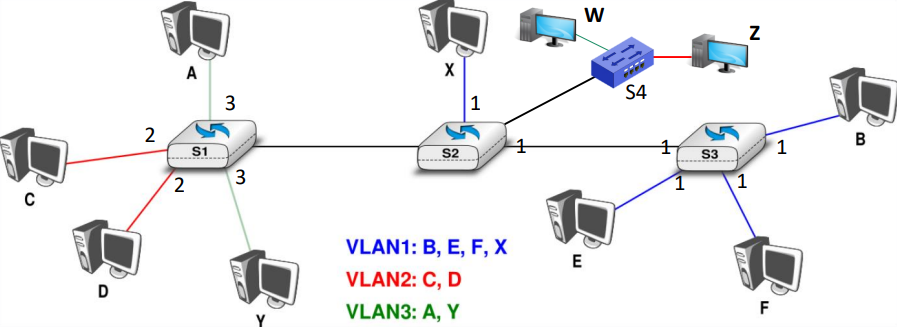
\includegraphics[width=\textwidth]{vlan1.png}
    \caption{Esempio di rete con tre \emph{VLAN}}
\end{figure}\noindent
Dalla figura si vede come ogni interfaccia dei tre \emph{switch} sia associata
ad una \emph{VLAN} con l'unica eccezione delle porte alle quali si collega il
canale tra \emph{S1} e \emph{S2}. In quel caso le porte sono configurate in
modalità \emph{trunk} e ciò significa che permettono il passaggio del
traffico di più di una \emph{VLAN}.

C'è però un problema. Per poter capire a quale \emph{VLAN} appartiene ogni
\emph{frame} sarebbe necessario inserire un identificativo nell'header, ma
ciò non è possibile perché lo standard 802.3 di \emph{Ethernet} non consente
di inserire quest'informazione in nessuno dei campi già esistenti. Di
conseguenza, fu introdotta una modifica allo standard con la realizzazione
della versione 802.1Q di \emph{Ethernet}.

\bigskip\noindent
Con il nuovo standard furono introdotti quattro nuovi campi nell'header:
\begin{itemize}
    \item \texttt{VLAN protocol ID}: contiene un valore fisso a \texttt{0x8100};
    \item \texttt{Pri}: contiene il valore di priorità del \emph{frame} ed è
    usato per realizzare politiche di quality of service;
    \item \texttt{\gls{glos:CFI}}: inizialmente specificava se l'ordine dei
    byte era big endian o little endian, ma successivamente dalla versione 802.5
    fu utilizzato per reti a \emph{token passing};
    \item \texttt{VLAN identifier}: valore a 12 bit che identifica la \emph{VLAN}
    di appartenenza;
\end{itemize}

\begin{note}
    Nel campo \texttt{VLAN identifier} il valore \texttt{0} indica l'assenza di
    \emph{VLAN}, mentre \texttt{0xFFF} è riservato.
\end{note}
\begin{note}
    I campi \texttt{Pri}, \texttt{CFI} e \texttt{VLAN identifier} fanno parte
    in realtà di un unico campo logico chiamato \texttt{Tag}.
\end{note}\noindent
Esiste una forma di retrocompatibilità indiretta del nuovo standard col precedente.
In particolare, non è necessario che gli \emph{host} supportino le
\emph{VLAN}\footnotemark\! in quanto gli \emph{switch} possono manipolare i
\emph{frame} per aggiungere e togliere le informazioni necessarie. Quando una
porta di uno \emph{switch} riceve un \emph{frame} \quotes{non taggato} 
aggiunge i campi necessari specificando come \emph{VLAN ID} l'ID della
\emph{VLAN} associata a quella porta e allo stesso modo, quando deve inoltrare
un \emph{frame} verso un \emph{host}, rimuove i campi aggiuntivi.

\footnotetext{Gli \emph{host} possono non essere neanche a conoscenza
dell'esistenza delle \emph{VLAN}}

Se invece uno \emph{switch} che non supporta le \emph{VLAN} riceve un
\emph{frame} \quotes{taggato} ci sono due possibilità: nel caso peggiore, lo
\emph{switch} non riconosce il formato del \emph{frame} e quindi lo scarta. In
alternativa, se lo \emph{switch} conosce lo standard, ma non è stato configurato,
inoltra il \emph{frame} senza considerare le \emph{VLAN}.

Un \emph{host} che usa le \emph{VLAN} può inviare \emph{frame} con \emph{VLAN
ID} diversi a seconda del tipo di dati che sta trasmettendo.

\section{Organizzazione e funzionamento delle reti wireless}
\subsection{Elementi di una rete wireless}
Gli elementi fondamentali di una rete wireless sono tre:
\begin{itemize}
    \item \emph{Host wireless}: sono i dispositivi utente in grado di connettersi
    alla rete e possono essere sia statici che mobili;
    \item \emph{Stazione base}: è un dispositivo relay che fa da ponte tra la
    rete wireless e la rete cablata e infatti tipicamente è collegato ad una
    rete cablata;
    \item \emph{Collegamenti wireless}: sono i mezzi trasmissivi che permettono
    ad \emph{host} e \emph{stazioni base} di comunicare. L'accesso al mezzo è
    gestito da appositi protocolli \emph{\gls{prot:MACp}} e tipicamente, la
    \emph{velocità di trasmissione} diminuisce all'aumentare della distanza;
\end{itemize}
Le reti wireless sono realizzabili secondo due modalità:
\begin{itemize}
    \item \emph{Infrastrutturata}: le \emph{stazioni base} connettono gli
    \emph{host} alla rete cablata e con un'operazione di \emph{handover} gli
    \emph{host} mobili possono cambiare la \emph{stazione base} a cui
    collegarsi;
    \item \emph{Ad hoc}: non esistono \emph{stazioni base} e ogni \emph{host}
    può comunicare soltanto con gli altri \emph{host} all'interno del proprio
    raggio di copertura. Gli \emph{host} si connettono direttamente tra loro
    con un processo di scoperta automatica dei vicini;
\end{itemize}

\begin{figure}[ht!]
    \centering
    \subfloat[Rete wireless in modalità \emph{infrastrutturata}]{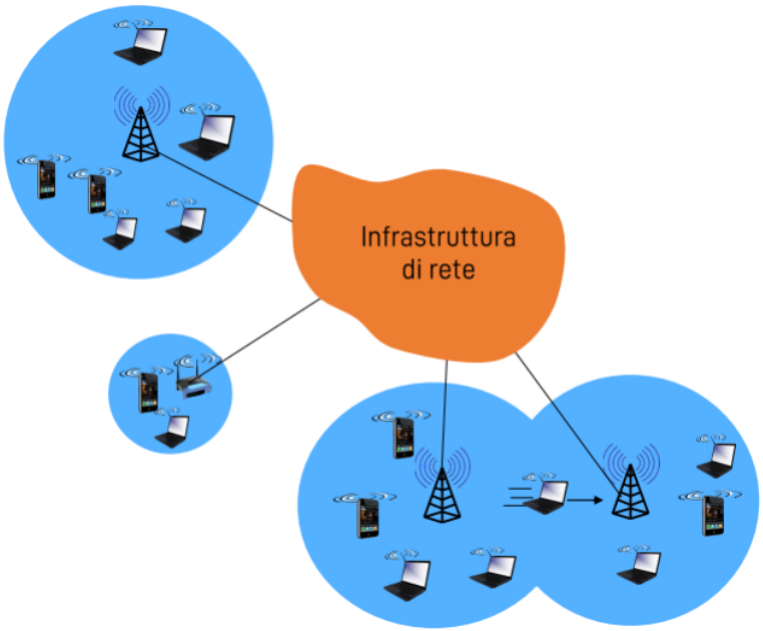
\includegraphics[width=0.58\textwidth]{wlan1.png}}
    \hfill
    \subfloat[Rete wireless in modalità \emph{ad hoc}]{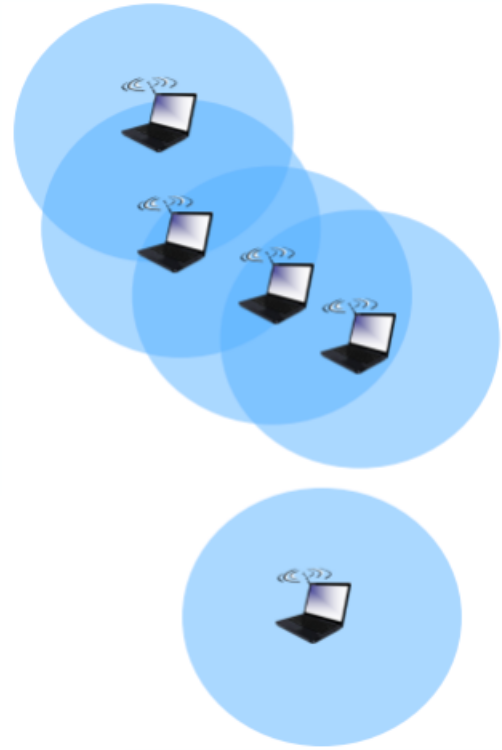
\includegraphics[width=0.4\textwidth]{wlan2.png}}
    \caption{Tipologie di reti wireless}
\end{figure}
\begin{note}
    Nelle reti wireless realizzate con modalità \emph{ad hoc} gli \emph{host}
    più distanti, che quindi non sono direttamente collegati tra loro,
    comunicano per mezzo di percorsi multi-salto.
\end{note}\noindent
Detto questo possiamo classificare le reti wireless sia in base al tipo di
infrastruttura che alla presenza o meno di percorsi multi-salto.
\begin{table}[h!]
    \centering
    \renewcommand{\arraystretch}{1.2}
    \begin{tabular}{|p{0.22\textwidth}|p{0.35\textwidth}|p{0.35\textwidth}|}
        \hline
         & \textbf{Non multi-salto} & \textbf{Multi-salto}\\
        \hline
        \textbf{Rete con modalità infrastrutturata} & L'\emph{host} si connette alla
        \emph{stazione base} che lo collega a internet & L'\emph{host}
        trasmette il messaggio attraverso altri \emph{host} prima di raggiungerne
        uno connesso a internet\\
        \hline
        \textbf{Rete con modalità ad hoc} & Non esiste nessuna \emph{stazione base} e quindi
        nessun \emph{host} può connettersi ad internet & Comunque non è possibile
        connettersi ad internet, ma la destinazione potrebbe lo stesso essere
        raggiunta\\
        \hline
    \end{tabular}
\end{table}

\subsection{Architettura di riferimento}
Solitamente le reti \emph{\gls{glos:WLAN}} costruite con la modalità
\emph{infrastrutturata} si basano su un'architettura standard. Secondo questo
modello di riferimento, tutti gli \emph{host} e le \emph{stazioni base} vengono
chiamati \emph{STA}. Gruppi di \emph{STA} che usano lo stesso canale vengono
raggruppati all'interno di un \emph{\gls{glos:BSS}}. In ogni \emph{BSS} è
presente un \emph{\gls{glos:AP}} che è un dispositivo in grado di connettere
gli \emph{STA} di un \emph{BSS} al sistema di distribuzione, il quale, fornisce
connettività verso altri \emph{BSS} e, mediante un portale, anche verso internet.
Infine, gruppi di \emph{BSS} possono essere aggregati in un \emph{\gls{glos:ESS}}
a formare un'unica rete logica.

\begin{figure}[h!]
    \centering
    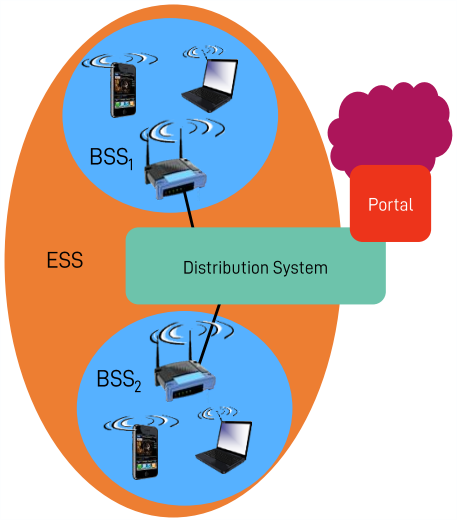
\includegraphics[width=0.5\textwidth]{architettura-wlan.png}
    \caption{Architettura di riferimento delle \emph{WLAN}}
\end{figure}\noindent
Specificando maggiormente, possiamo affermare che un \emph{BSS} sia un insieme
di \emph{STA} che usano lo stesso protocollo \emph{MAC} e competono per
l'accesso allo stesso mezzo trasmissivo. I protocolli \emph{MAC} possono
funzionare in modo distribuito o essere controllati dagli \emph{AP} che, di
fatto, funzionano come degli \emph{switch}. Inoltre, tutti gli \emph{STA}
vedono il proprio \emph{ESS} come un'unica rete e quindi non sono consapevoli
della divisione in \emph{BSS}.

\begin{note}
    I \emph{BSS} possono essere isolati disattivando o rimuovendo i suoi
    \emph{AP}.
\end{note}

\subsection{Protocolli per le comunicazioni wireless}
Le comunicazioni wireless sono regolate dallo standard 802.11b che suddivide
lo spettro di frequenze tra 2.4GHz e 2.485GHz in 11 canali. L'amministratore di
ogni \emph{AP} sceglie uno di quei canali e, se due \emph{AP} vicini scelgono lo
stesso, si creano interferenze. A quel punto gli \emph{host} si devono associare
ad un \emph{AP} e, per farlo, rimangono in ascolto, su tutti i canali, alla
ricerca di \emph{frame} particolari chiamatati \emph{\quotes{beacon}}. Un
\emph{beacon} contiene un \emph{\gls{glos:SSID}}, ovvero il nome di una rete,
e l'\emph{indirizzo MAC} dell'\emph{AP} che l'ha inviato. A quel punto,
l'\emph{host} sceglie a quale \emph{AP} associarsi, eventualmente autenticandosi,
e mediante \emph{\gls{prot:DHCP}} si fa assegnare un \emph{indirizzo IP} di
quella sottorete.

In realtà esistono due modalità di ricerca degli \emph{AP}: \emph{attiva} e
\emph{passiva}. Nella modalità \emph{attiva}, un \emph{host} invia a tutti i
vicini un \emph{frame} di \emph{probe request} e tutti gli \emph{AP} rispondono
con una \emph{probe response}. Nella modalità \emph{passiva} invece, gli \emph{AP}
trasmettono i \emph{beacon} e gli \emph{host} rispondono inviando una
richiesta di associazione all'\emph{AP} scelto, il quale, a sua volta, risponde
con un \emph{frame} di conferma.

\begin{figure}[ht!]
    \centering
    \subfloat[Modalità \emph{passiva}]{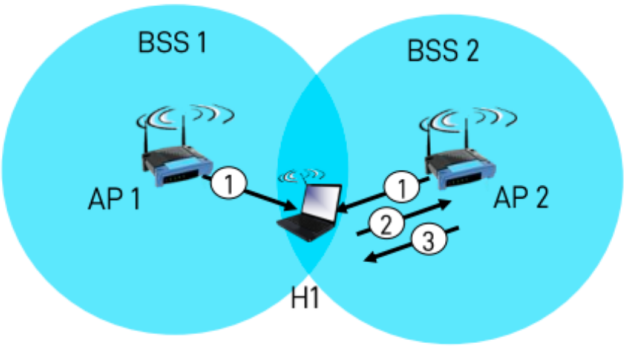
\includegraphics[width=0.48\textwidth]{ap-passiva.png}}
    \hfill
    \subfloat[Modalità \emph{attiva}]{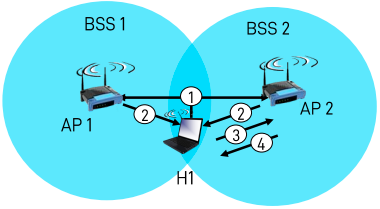
\includegraphics[width=0.48\textwidth]{ap-attiva.png}}
    \caption{Modalità di associazione degli \emph{host} con gli \emph{AP}}
\end{figure}

\newpage
\paragraph{Struttura di un frame wireless}
La struttura dei \emph{frame} per reti wireless è molto diversa dal
corrispettivo per reti cablate.

\begin{figure}[h!]
    \centering
    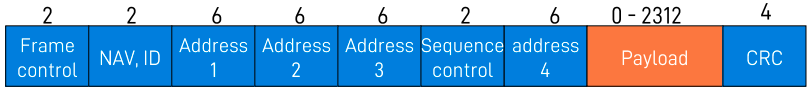
\includegraphics[width=0.8\textwidth]{frame-wireless.png}
    \caption{Struttura di un \emph{frame} 802.11}
\end{figure}\noindent
Vediamo l'impiego di alcuni di questi campi:
\begin{itemize}
    \item \texttt{Nav}: serve a specificare il tempo per il quale il
    canale rimarrà occupato;
    \item \texttt{Address 1}: \emph{indirizzo MAC} di destinazione;
    \item \texttt{Address 2}: \emph{indirizzo MAC} sorgente;
    \item \texttt{Address 3}: \emph{indirizzo MAC} dell'interfaccia del
    \emph{router} al quale l'\emph{AP} è collegato;
    \item \texttt{Address 4}: è utilizzato soltanto nelle reti wireless
    \emph{ad hoc};
\end{itemize}

\paragraph{Caratteristiche dei collegamenti wireless}
È bene esplicitare il fatto che la comunicazione wireless è molto più difficile
da realizzare rispetto alla controparte cablata. Il motivo, è che la potenza dei
segnali radio tende ad attenuarsi molto durante la propagazione e quindi, i
segnali arrivano a destinazione con una potenza minore. Inoltre, i segnali
radio sono anche sottoposti a forti interferenze da altri dispositivi e a
riflessioni che ne causano duplicazioni e sfasamenti.

\paragraph{Problemi nel rilevamento delle collisioni}
Per le ragioni espresse poc'anzi, la \emph{collision detection} non è possibile
nelle reti wireless e per capirne meglio il motivo può essere utile spiegare a
grandi linee come si propagano i segnali radio. Quando un'antenna trasmette,
il segnale si estende come sfere di raggio crescente a partire dall'antenna.
Di conseguenza, la potenza impressa dall'antenna deve distribuirsi su
superfici sempre più grandi la cui area cresce come il quadrato del raggio.
L'attenuazione segue quindi una legge quadratica:
\[P_{rx}=k\cdot\frac{P_{tx}}{d^2}\]
dove $d$ è il raggio della sfera, cioè la distanza dall'antenna, e $k$ è una
costante, tipicamente minore di 1, che conteggia altri fattori di attenuazione.

\noindent
Un'altra cosa che va compresa, è che un'antenna non può trasmettere e riceve
contemporaneamente e che se in un singolo \emph{AP} si mettessero due antenne,
si verificherebbero autointerferenze. Se ad esempio considerassimo un \emph{AP}
con due antenne, una trasmittente e una ricevente, la ricevente capterebbe
sia il segnale di un \emph{STA} della rete che il segnale dell'altra antenna.
Ovviamente, essendo la seconda antenna dell'\emph{AP} molto più vicina alla
ricevente, il suo segnale potrebbe interferire, o potenzialmente oscurare,
quello proveniente dall'\emph{STA}.

\subsection{Collision avoidance nelle reti wireless}
Abbiamo visto che non possiamo implementare la \emph{collision detection} nelle
reti wireless, quindi, l'unica alternativa è la \emph{collision avoidance}.
Infatti, il protocollo \emph{MAC} 802.11 è basato su \emph{\gls{prot:CSMA}} con
\emph{collision avoidance}. Gli \emph{STA} devono contendersi l'accesso al
canale ogni volta che intendono trasmettere.
\begin{note}
    In alcune versioni più avanzate di 802.11 è possibile concedere il canale
    a un \emph{STA} per un periodo di tempo più lungo di un \emph{frame}.
    Questo periodo è detto \emph{TXOP} e permette al trasmettitore di inviare
    più \emph{frame} in sequenza.    
\end{note}\noindent
Quindi, vediamo nel dettaglio con un esempio il processo di contesa.

\begin{eg}[Esempio di funzionamento del protocollo MAC 802.11]
    Supponiamo che \texttt{STA 1} e \texttt{STA 2} debbano trasmettere un frame
    all'AP. Entrambi i contendenti rimangono in ascolto sul canale fino a
    quando questo non viene percepito libero per un tempo pari a un
    \gls{glos:DIFS}. A quel punto, entrambi estraggono a caso un backoff
    tra 0 e $\gls{glos:CW}-1$ e si mettono in attesa.

    Supponiamo che \texttt{STA 1} e \texttt{STA 2} abbiano scelto un backoff di
    3 e 5 rispettivamente.

    \begin{figure}[h!]
        \centering
        \subfloat[Situazione iniziale]{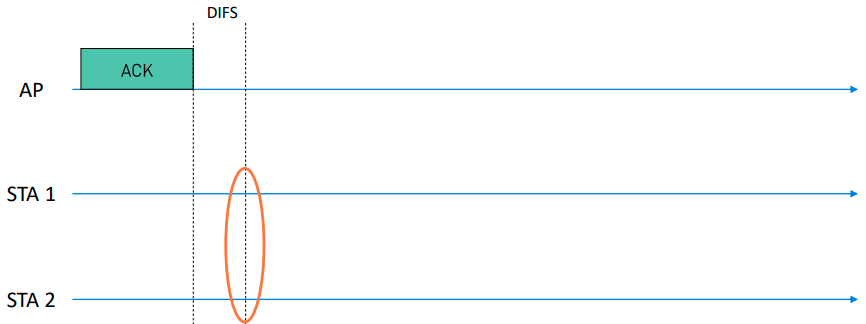
\includegraphics[width=0.48\textwidth]{csma-ca-1.png}}
        \hfill
        \subfloat[Scelta dei backoff]{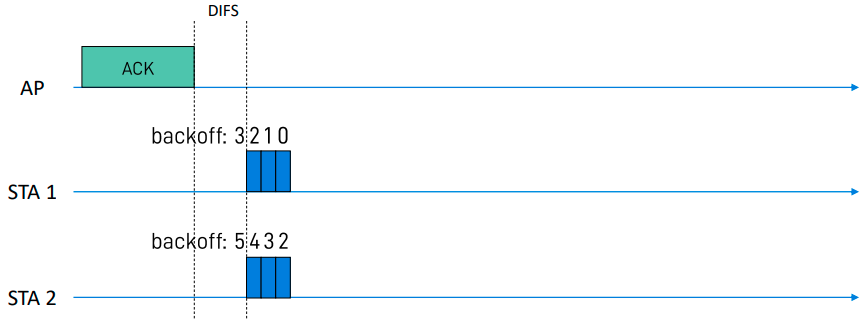
\includegraphics[width=0.48\textwidth]{csma-ca-2.png}}
    \end{figure}\noindent
    Allo scadere del backoff di \texttt{STA 1}, \texttt{STA 1} testa il canale
    e, siccome è libero, trasmette l'intero frame. Quando l'AP ha ricevuto
    l'intero frame rimane in attesa per un \gls{glos:SIFS}\,\footnotemark e
    quindi risponde con un \gls{glos:ACK}. Quando \texttt{STA 1} inizia a
    trasmettere, \texttt{STA 2} percepisce che il canale è occupato, quindi
    congela l'attuale valore di backoff e si mette in attesa per un tempo pari
    al valore scritto nel campo \texttt{NAV} dell'header del frame trasmesso da
    \texttt{STA 1}.
    \begin{figure}[h!]
        \ContinuedFloat
        \centering
        \subfloat[\texttt{STA 1} trasmette]{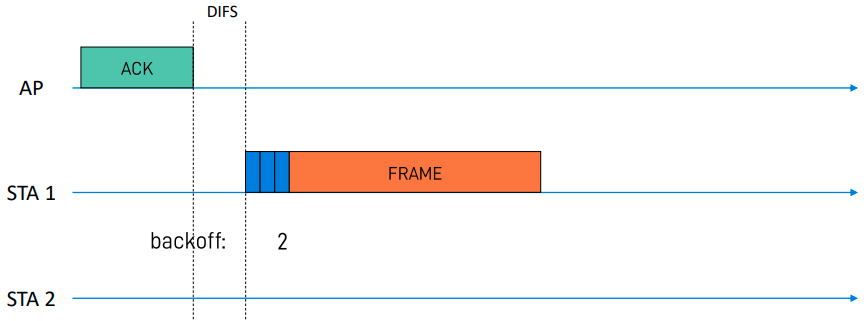
\includegraphics[width=0.48\textwidth]{csma-ca-3.png}}
        \hfill
        \subfloat[L'AP risponde con un ACK]{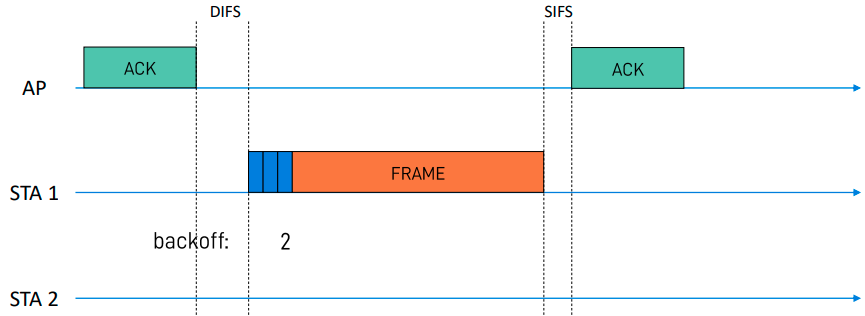
\includegraphics[width=0.48\textwidth]{csma-ca-4.png}}
    \end{figure}

    \newpage\noindent
    Allo scadere dell'attesa, del backoff e dopo aver lasciato passare un DIFS,
    se il canale è libero, \texttt{STA 2} trasmette il proprio frame.
    \begin{figure}[h!]
        \ContinuedFloat
        \centering
        \subfloat[\texttt{STA 2} trasmette]{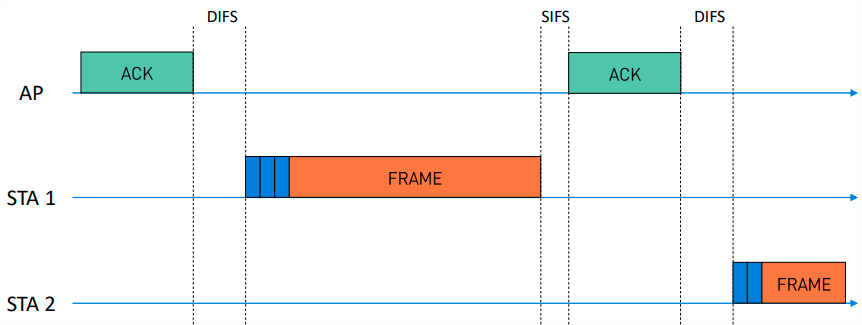
\includegraphics[width=0.48\textwidth]{csma-ca-5.png}}
    \end{figure}

    \bigskip\noindent
    Ma cosa sarebbe successo se \texttt{STA 1} e \texttt{STA 2} avessero scelto
    lo stesso valore di backoff?

    Semplicemente, avrebbero iniziato a trasmettere nello stesso momento, si
    sarebbe verificata una collisione, ma senza che i due trasmettitori se ne
    rendessero conto. L'AP non riuscendo a ricevere nessuno dei due frame, non
    avrebbe trasmesso nessun ACK e quindi, dopo un DIFS, \texttt{STA 1} e
    \texttt{STA 2} avrebbero raddoppiato la $CW$ e ripetuto la procedura vista
    in precedenza.
\end{eg}
\footnotetext{$\emph{SIFS}<\emph{DIFS}$}
\begin{note}
    Nelle reti wireless l'utilizzo degli \emph{ACK} è necessario perché
    tra \emph{collisioni}, errori di trasmissione e il problema del terminale
    nascosto è molto più probabile che i \emph{frame} non arrivino a destinazione
    e, non essendo possibile rilevare le \emph{collisioni}, è necessario avvisare
    il mittente dell'avvenuta consegna.
\end{note}

\subsection{Problema del terminale nascosto}
Alla fine della precedente sottosezione abbiano nominato il \quotes{problema
del terminale nascosto}. Questo problema si verifica quando si hanno degli
\emph{STA} che vedono dei vicini comuni, ma non si vedono tra loro a causa di
ostacoli o forti attenuazioni di segnale. Ciò può portare al verificarsi di
\emph{collisioni} sugli \emph{STA} comuni.

\begin{figure}[h!]
    \centering
    \subfloat{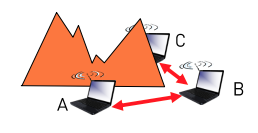
\includegraphics[width=0.48\textwidth]{terminale-nascosto-1.png}}
    \subfloat{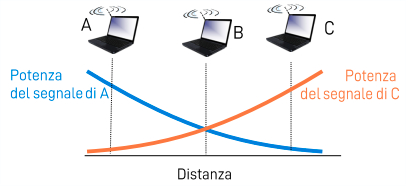
\includegraphics[width=0.48\textwidth]{terminale-nascosto-2.png}}
    \caption{$A$ e $C$ vedono entrambi $B$, ma non si vedono tra loro}
\end{figure}\noindent
Per evitare ciò, viene introdotta una procedura di \emph{handshake}
nel \emph{CSMA/CA}. La fase di \emph{handshake} serve per prenotare esplicitamente
il canale e prevede lo scambio di due messaggi preliminari. L'\emph{STA}
intenzionato a trasmettere invia un \emph{\gls{glos:RTS}} e il ricevitore
risponde con un \emph{\gls{glos:CTS}}. Il messaggio \emph{CTS} serve sia a
prenotare il canale per il trasmettitore che a notificare agli altri \emph{STA}
un'imminente trasmissione. Questo mitiga il problema del terminale nascosto al
prezzo di un overhead maggiore.

\begin{note}
    \emph{RTS} e \emph{CTS} sono messaggi brevi e se anche collidessero, la
    \emph{collisione} durerebbe per meno tempo e verrebbero sprecate meno
    risorse radio.
\end{note}

\newpage
\begin{figure}[ht!]
    \centering
    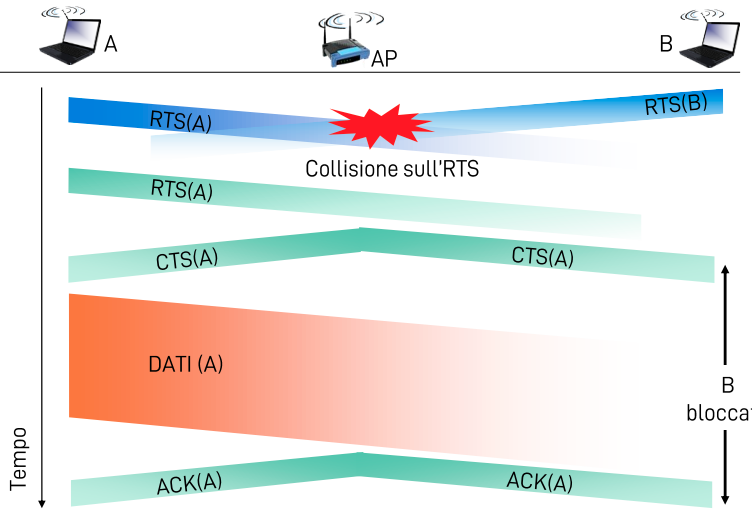
\includegraphics[width=0.7\textwidth]{terminale-nascosto-3.png}
    \caption{Risoluzione del problema del terminale nascosto}
\end{figure}

\bigskip\noindent
Questa soluzione introduce però un ulteriore problema: il problema del terminale
esposto.

\begin{figure}[h!]
    \centering
    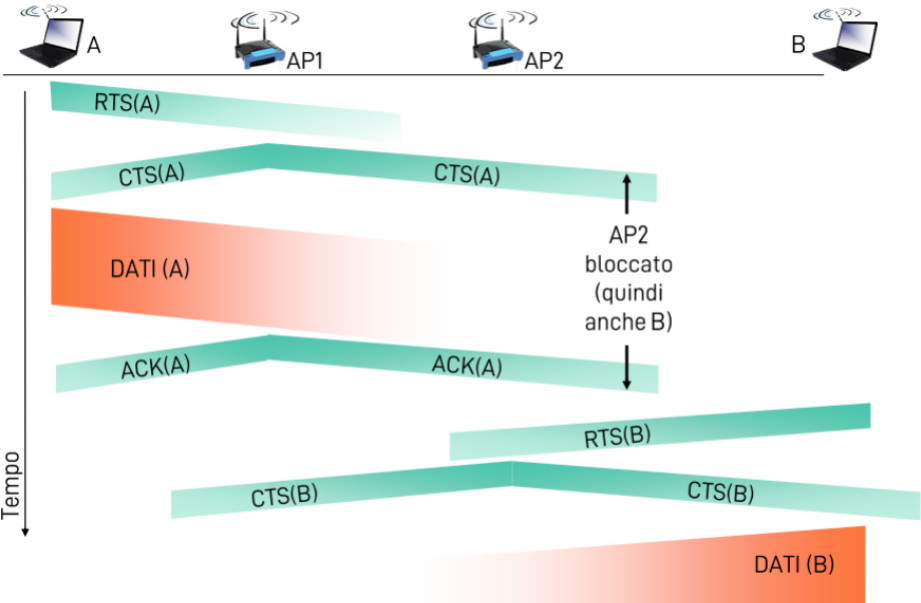
\includegraphics[width=0.7\textwidth]{terminale-esposto.png}
    \caption{Problema del terminale esposto}
\end{figure}\noindent
Nella situazione rappresentata nella figura di cui sopra, ad esempio, $B$ è
costretto a rimanere in attesa mentre $A$ comunica con $AP1$. L'attesa però è
inutile in quanto $B$ avrebbe potuto comunicare con $AP2$ senza provocare
interferenze né \emph{collisioni} su $AP1$.

A questo problema collaterale non esiste al momento una soluzione, ma lo si
accetta perché il problema del terminale nascosto è più grave.